% !TeX program = pdflatex
\documentclass[tikz,border=8pt]{standalone}
\usepackage{pgfplots}
\pgfplotsset{compat=1.16}
\definecolor{FigureBlue}{HTML}{2563EB}
\definecolor{FigureOrange}{HTML}{EA580C}
\definecolor{FigureSlate}{HTML}{475569}
\begin{document}
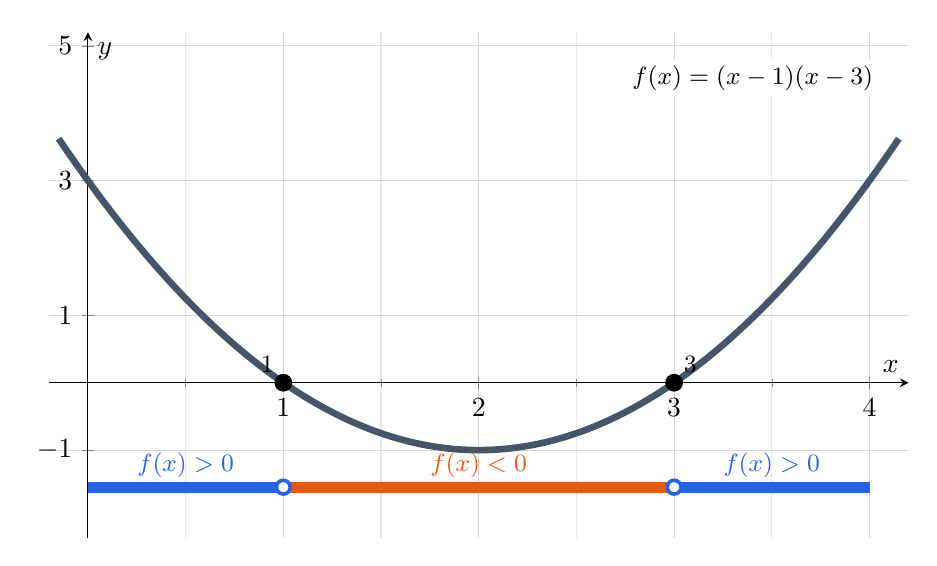
\begin{tikzpicture}
  \begin{axis}[
    width=12.5cm,height=8cm,axis lines=middle,
    xmin=-.2,xmax=4.2,ymin=-2.3,ymax=5.2,
    xlabel={$x$},ylabel={$y$},xtick={0,1,2,3,4},ytick={-1,0,1,3,5},
    grid=both,minor tick num=1,grid style={draw=gray!18},major grid style={draw=gray!32},clip=false,
  ]
    \addplot[FigureSlate,line width=2.4pt,domain=-.15:4.15,samples=181] {(x-1)*(x-3)};
    \addplot[only marks,mark=*,mark size=3pt,black] coordinates {(1,0) (3,0)};
    \draw[FigureBlue,line width=4pt] (axis cs:0,-1.55)--(axis cs:1,-1.55);
    \draw[FigureBlue,line width=4pt] (axis cs:3,-1.55)--(axis cs:4,-1.55);
    \draw[FigureOrange,line width=4pt] (axis cs:1,-1.55)--(axis cs:3,-1.55);
    \draw[fill=white,draw=FigureBlue,line width=1.3pt] (axis cs:1,-1.55) circle[radius=2.5pt];
    \draw[fill=white,draw=FigureBlue,line width=1.3pt] (axis cs:3,-1.55) circle[radius=2.5pt];
    \node[anchor=south,text=FigureBlue,font=\small] at (axis cs:.5,-1.55) {$f(x)>0$};
    \node[anchor=south,text=FigureOrange,font=\small] at (axis cs:2,-1.55) {$f(x)<0$};
    \node[anchor=south,text=FigureBlue,font=\small] at (axis cs:3.5,-1.55) {$f(x)>0$};
    \node[anchor=south east,font=\small] at (axis cs:1,0) {$1$};
    \node[anchor=south west,font=\small] at (axis cs:3,0) {$3$};
    \node[anchor=north east,fill=white,inner sep=2pt,font=\small]
      at (axis cs:4.05,4.8) {$f(x)=(x-1)(x-3)$};
  \end{axis}
\end{tikzpicture}
\end{document}
